\documentclass[margin=1pt]{standalone}

\usepackage{tikz}

\usetikzlibrary{
  calc, math,
  arrows, arrows.meta,
  decorations.pathreplacing,
  calligraphy,
}

\begin{document}
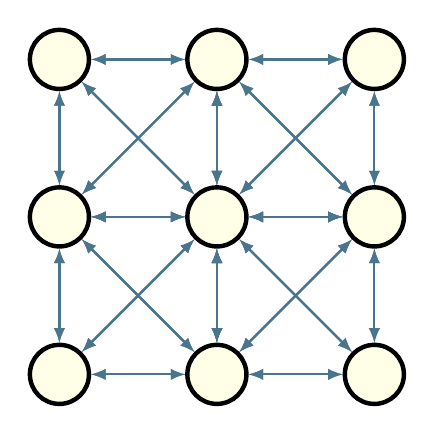
\begin{tikzpicture}[
    ultra thick,
    arr/.style={thick, cyan!50!black},
    lab/.style={font=\ttfamily, black},
    circ/.style={fill=yellow!10, draw=black, circle, minimum size=7.5mm},
  ]
  \foreach \i in {0,1,2} {
      \foreach \j in {0,1,2}{
          \node[circ] (w\i\j) at (2*\i,-2*\j) {};
        }
    }
  \foreach \a/\b in {0/0,0/1,1/0,1/1} {
      \foreach \ia in {0,1} {
          \foreach \ib in {0,1} {
              \foreach \ja in {0,1} {
                  \foreach \jb in {0,1} {
                      \ifx\ia\ib
                        \ifx\ja\jb
                        \else
                          \draw[
                            evaluate={
                                \xa = int(\ia + \a);
                                \xb = int(\ib + \a);
                                \ya = int(\ja + \b);
                                \yb = int(\jb + \b);
                              },
                            latex-latex, arr
                          ] (w\xa\ya) -- (w\xb\yb);
                        \fi
                      \else
                        \draw[
                          evaluate={
                              \xa = int(\ia + \a);
                              \xb = int(\ib + \a);
                              \ya = int(\ja + \b);
                              \yb = int(\jb + \b);
                            },
                          latex-latex, arr
                        ] (w\xa\ya) -- (w\xb\yb);
                      \fi
                    }
                }
            }
        }
    }
\end{tikzpicture}
\end{document}
